\documentclass[12pt]{article}

\usepackage[utf8]{inputenc}
\usepackage{datetime}
\usepackage{amsthm}
\usepackage{amsmath}
\usepackage{amssymb}
\usepackage{enumitem}
\usepackage[USenglish]{babel}
\usepackage{matlab-prettifier}
\usepackage{graphicx}

\newcommand\independent{\protect\mathpalette{\protect\independenT}{\perp}}
\def\independenT#1#2{\mathrel{\rlap{$#1#2$}\mkern2mu{#1#2}}}

\newtheoremstyle{colon}{\topsep}{\topsep}{}{}{\bfseries}{:}{ }{}
\theoremstyle{colon}
\newtheorem{exercise}{Exercise}
\newtheorem*{answer}{Answer}

\title{ORFE 524: Statistical Theory and Methods \\ Homework 6}
\author{Zachary Hervieux-Moore}

\newdate{date}{16}{12}{2016}
\date{\displaydate{date}}

\begin{document}
\maketitle

\clearpage

\begin{exercise}
  Suppose that $\widehat{\theta}_n$ is a bounded estimator of $\theta$ (that is, $\lvert \widehat{\theta}_n \rvert \leq B, \forall n$ for some $B$). Show that if $a_n(\widehat{\theta}_n - \theta) \xrightarrow{d} X$ with $a_n \rightarrow \infty$, then $\widehat{\theta}_n$ is $L_2$-consistent (i.e. $\mathbb{E}[\lvert \widehat{\theta}_n - \theta \rvert^2] \rightarrow 0$)
\end{exercise}

\begin{answer}
  We have that $\mathbb{E}[\lvert \widehat{\theta}_n - \theta \rvert^2] \rightarrow 0$ is equivalent to $\mathbb{E}[\widehat{\theta}_n^2 + \theta^2] \rightarrow 2 \mathbb{E}[\widehat{\theta}_n \theta]$. So we apply Delta theorem with $g(\theta) = \theta^2$. So,
  \begin{gather*}
    a_n(\widehat{\theta}_n^2 - \theta^2) \xrightarrow{d} \frac{d}{d \theta} \theta^2 \cdot X \\
    \Longleftrightarrow a_n(\widehat{\theta}_n^2 - \theta^2) \xrightarrow{d} 2 \theta X \\
    \Longleftrightarrow \widehat{\theta}_n^2 + \theta^2 \xrightarrow{d} \frac{2 \theta X}{a_n} + 2 \theta^2
  \end{gather*}
  Now, note that
  \begin{gather*}
    a_n(\widehat{\theta}_n - \theta) \xrightarrow{d} X \\
    \Longleftrightarrow \widehat{\theta}_n \xrightarrow{d} \frac{X}{a_n} + \theta \\
    \Longleftrightarrow 2\widehat{\theta}_n \theta \xrightarrow{d} \frac{2 \theta X}{a_n} + 2 \theta^2
  \end{gather*}
  So,
  \begin{gather*}
    a_n(\widehat{\theta}_n^2 - \theta^2) \xrightarrow{d} \frac{2 \theta X}{a_n} + 2 \theta^2 \\
    \Longleftrightarrow \widehat{\theta}_n^2 + \theta^2 \xrightarrow{d} 2 \widehat{\theta}_n \theta
  \end{gather*}
  Taking expectations gives us the result.
\end{answer}

\clearpage

\begin{exercise}
  Let $X \sim P$ be a random variable satisfying $\mathbb{E}[X] = \mu$, $\mathbb{E}[X^2] < \infty$. Let $x = \{ x_i \}_{i = 1}^n$ be $n$ i.i.d. observations of $X$. Consider test function
  \begin{gather*}
    T(x) = \{ x : \frac{\sqrt{n} \lvert \bar{x} - \mu_0 \rvert }{S_n} \geq z_{\alpha/2} \}
  \end{gather*}
  for hypothesis testing problem $H_0 : \mu = \mu_0$ versus $H_1 : \mu \neq \mu_0$, where $z_{\alpha/2}$ is the $(1 - \alpha/2)$-quantile of $N(0,1)$. Derive the asymptotic power of this test, i.e. find the limit of $\beta_n(\mu)$ as $n \rightarrow \infty$. Recall that $\beta_n(\mu) := P(T(X) = 1)$ when the expectation of $X$ is $\mu$.
\end{exercise}

\begin{answer}
  We have by Slutsky's theorem that
  \begin{gather*}
    \frac{\sqrt{n} (\bar{x} - \mu) }{S_n} \rightarrow N(0,1)
  \end{gather*}
  Thus, we have that
  \begin{gather*}
    \lim_{n \rightarrow \infty} \beta_n(\mu) = \lim_{n \rightarrow \infty} P(T(X) = 1) \\
    = 1 - \lim_{n \rightarrow \infty} P \left( -z_{\alpha/2} \geq \frac{\sqrt{n} \bar{x} - \mu_0}{S_n} \leq z_{\alpha/2} \right) \\
    = 1 - \lim_{n \rightarrow \infty} P \left( -z_{\alpha/2} \geq \frac{\sqrt{n} \bar{x} - \mu + \mu - \mu_0}{S_n} \leq z_{\alpha/2} \right) \\
    = 1 - \lim_{n \rightarrow \infty} P \left( -z_{\alpha/2}/\sqrt{n} \geq \frac{ \bar{x} - \mu }{S_n} + \frac{\mu - \mu_0}{S_n} \leq z_{\alpha/2}/\sqrt{n} \right)
  \end{gather*}
  However, we have by the central limit theorem we have that this converges to
  \begin{gather*}
    = 1 - \lim_{n \rightarrow \infty} P \left( -z_{\alpha/2}/\sqrt{n} \geq \frac{\mu - \mu_0}{\sigma} \leq z_{\alpha/2}/\sqrt{n} \right)
  \end{gather*}
  Thus, the power is tends to 1 as $n \rightarrow \infty$, because the probability term goes to 0.
\end{answer}

\clearpage

\begin{exercise}
  Let $X \sim P_X$ and $Y \sim P_Y$ be two independent random variables with $\mathbb{E}[X] = \mu_X$, $\mathbb{E}[Y] = \mu_Y$ and $\mathbb{E}[X^2] < \infty$, $\mathbb{E}[Y^2] < \infty$. We assume that both $\mu_X$ abd $\mu_Y$ are nonzero. Let $\{ x_i \}_{i=1}^n$ and $\{ y_i \}_{i=1}^n$ be $n$ i.i.d. copies of $X$ and $Y$, respectively. Consider the hypothesis testing problem $H_0 : \mu_X = \mu_Y$ versus $H_1 : \mu_X \neq \mu_Y$. Derive a test of asymptotic level $\alpha$ using statistic $\bar{x} / \bar{y}$. (Hint: rewrite the hypothesis testing problem using $\mu_X / \mu_Y$).
\end{exercise}

\begin{answer}
  We first rewrite the hypothesis testing problem as $H_0 : \mu_X/\mu_Y = 1$ versus $H_1 : \mu_X/\mu_Y \neq 1$. Now, we note that $\bar{y} \xrightarrow{p} \mu_Y$ by the Law of Large Numbers. Also, $\sqrt{n}(\bar{x} - \mu_X)/S_n \xrightarrow{d} N(0, 1)$ by Central Limit Theorem. Thus, using $h(x, y) = \frac{x}{y}$ and applying Slutky's theoream, we get
  \begin{gather*}
    \frac{\sqrt{n}(\bar{x} - \mu_X)}{S_n \cdot \bar{y}} \xrightarrow{d} \frac{N(0, 1)}{\mu_Y}
  \end{gather*}
  Thus, the following test has asymptotic level $\alpha$
  \begin{gather*}
    T(x, y) = \{ x,y : \frac{\sqrt{n} \lvert \bar{x} - \mu_X \rvert}{S_n \cdot \bar{y}} \geq z_{\alpha/2}/\mu_Y^2 \}
  \end{gather*}
\end{answer}

\clearpage

\begin{exercise}
  Suppose $X \sim P$ is a random variable with $\mathbb{E}[X] = \mu \neq 0$ and $\mathbb{E}[X^2] < \infty$ unknown. Let $x = \{ x_i \}_{i=1}^n$ be $n$ i.i.d. observations of $X$.
  \begin{enumerate}[label=\arabic*)]
    \item Derive an $(1-\alpha)$-level asymptotic confidence interval for $1/\mu$. Your interval should be proper, i.e. not depend on unknowns. Argue every step.
    \item Invert the above confidence interval to obtain a test for
      \begin{gather*}
        H_0 : \mu < 0 \text{ or } \mu \geq 1/2 \text{ versus } H_1 : 0 < \mu < 1/2
      \end{gather*}
  \end{enumerate}
\end{exercise}

\begin{answer}
  \leavevmode
  \begin{enumerate}[label=\arabic*)]
    \item We have by central limit theorem that
      \begin{gather*}
        \sqrt{n} \frac{\bar{x} - \mu}{\sigma} \rightarrow N(0,1)
      \end{gather*}
      Now, applying the Delta theorem using $g(x) = 1/x$, we have
      \begin{gather*}
        \sqrt{n} \frac{1/\bar{x} - 1/\mu}{\sigma} \rightarrow N(0,1/\mu^2)
      \end{gather*}
      Hence, by Slutsky's theorem, we have
      \begin{gather*}
        \sqrt{n} \frac{1/\bar{x} - 1/\mu}{\bar{\sigma}/\bar{x}^2} \rightarrow N(0,1)
      \end{gather*}
      Thus, picking the normal confidence test,
      \begin{gather*}
        \lim_{n \rightarrow \infty} P \left( \sqrt{n} \frac{\lvert 1/\bar{x} - 1/\mu \rvert}{\bar{\sigma}/\bar{x}^2} \leq z_{\alpha/2} \right) \rightarrow 1 - \alpha
      \end{gather*}
      The interval becomes $\frac{1}{\bar{x}} \pm \frac{z_{\alpha/2} \bar{\sigma}}{\sqrt{n} \bar{x}^2}$
    \item Inverting the test yields
      \begin{gather*}
        H_0 : 1/\mu \leq 2 \text{ versus } H_1 : 1/\mu > 2
      \end{gather*}
      Thus, using the previous part, the test for this becomes
      \begin{gather*}
        T(x) = \{ x : \frac{1}{\bar{x}} - \frac{z_{\alpha/2} \bar{\sigma}}{\sqrt{n} \bar{x}^2} > 2 \}
      \end{gather*}
  \end{enumerate}
\end{answer}

\clearpage

\begin{exercise}
  Consider the kernel density estimator based on i.i.d. observation $\{ x_i \}_{i=1}^n$ of $X$ in $\mathbb{R}^d$. Fix $x_0 \in \mathbb{R}^d$. For simplicity we assume that $K$ is symmetric and bounded kernel. Suppose that the density of $X$, denoted $f$, is bounded and uniformly continuous in $\mathbb{R}^d$. Recall that a kernel density estimator is
  \begin{gather*}
    \widehat{f}_h(x) = \frac{1}{n h^d} \sum_i K \left( \frac{x - x_i}{h} \right)
  \end{gather*}
  \begin{enumerate}[label=\arabic*)]
    \item Show that the bias $\mathbb{E}[\widehat{f}_h(x_0) - f(x_0)] \xrightarrow{h \rightarrow 0} 0$. (Hint: express the expectation as an integral involving $K(u)$).
    \item Define $K = \int K^2(u) du$ and suppose that there exists $F > 0$ satisfying $\sup_x f(x) \leq F$. Find an upper bound of var($\widehat{f}_h(x_0)$) in terms of $K$ and $F$.  Conclude that if $n \rightarrow \infty$ and $h \rightarrow 0$ with $n h^d \rightarrow \infty$, then $\mathbb{E}[\lvert \widehat{f}_h(x_0) - f(x_0) \rvert^2] \rightarrow 0$.
  \end{enumerate}
\end{exercise}

\begin{answer}
  \leavevmode
  \begin{enumerate}[label=\arabic*)]
    \item We have that
      \begin{gather*}
        \lim_{h \rightarrow 0} \mathbb{E}[\widehat{f}_h(x_0) - f(x_0)] \\
        = \lim_{h \rightarrow 0} \int \frac{1}{n h^d} \sum_i K \left( \frac{x_0 - x_i}{h} \right) - f(x_0) dP(x) \\
        = \lim_{h \rightarrow 0} \frac{1}{n h^d} \sum_i \int K \left( \frac{x_0 - x_i}{h} \right) dP(x) - f(x_0) \int dP(x)
      \end{gather*}
      Since the $x_i$ are i.i.d. we can go to the single vector case
      \begin{gather*}
        = \lim_{h \rightarrow 0} \frac{1}{h^d} \int_{\mathbb{R}^d} K \left( \frac{x_0 - x}{h} \right) dP(x) - f(x_0)
      \end{gather*}
      Let $u = \frac{x_0 - x}{h} = \frac{x - x_0}{h}$ since $K$ is symmetric. So $dx = h^d du$. Making the substitution,
      \begin{gather*}
        = \lim_{h \rightarrow 0} \frac{1}{h^d} \int_{\mathbb{R}^d} K(u) h^d f(x_0 - hu) du - f(x_0) \\
        = \lim_{h \rightarrow 0} \int_{\mathbb{R}^d} K(u) f(x_0 - hu) du - f(x_0)
      \end{gather*}
      Since $K$ and $f$ are both bounded and $K$ is integrable, then we can use Dominated Convergence Theorem (picking $K(u)B$ as the dominating function) to bring in the limit. It is a Kernel, so it also integrals to 1. Finally, we can take the limit inside $f$ as it is continuous. So,
      \begin{gather*}
        = \int_{\mathbb{R}^d} K(u) \lim_{h \rightarrow 0} f(x_0 - hu) du - f(x_0) \\
        = \int_{\mathbb{R}^d} K(u) f(\lim_{h \rightarrow 0} x_0 - hu) du - f(x_0) \\
        = f(x_0) \int_{\mathbb{R}^d} K(u) du - f(x_0) \\
        = f(x_0) - f(x_0) = 0
      \end{gather*}
      Thus, $\mathbb{E}[\widehat{f}_h(x_0) - f(x_0)] = 0$ or equivalently, $\mathbb{E}[\widehat{f}_h(x_0)] = \mathbb{E}[f(x_0)]$.
    \item Calculating the variance,
      \begin{gather*}
        var(\widehat{f}_h(x_0)) = var \left(\frac{1}{h^d n} \sum_i K \left( \frac{x_0 - x}{h} \right) \right) \\
        = \frac{1}{h^{2d} n^2} \sum_i var \left(K \left( \frac{x_0 - x}{h} \right) \right) \\
        = \frac{1}{h^{2d} n} var\left(K \left( \frac{x_0 - x}{h} \right) \right)
      \end{gather*}
      Where the equality is a result of i.i.d.
      Now, upper bounding the variance by the expectation of the square,
      \begin{gather*}
        \leq \frac{1}{h^{2d} n} \mathbb{E}[K \left( \frac{x_0 - x}{h} \right)^2] \\
        = \frac{1}{h^{d} n} \mathbb{E}[K(u)^2]
        = \frac{K F}{h^d n}
      \end{gather*}
      Thus, given that the denomenator tends to infinity, then the variance goes to 0. Using the Variance-Bias decomposition and the two results shows that $\mathbb{E}[\lvert \widehat{f}_h(x_0) - f(x_0) \rvert^2] \rightarrow 0$ as well.
  \end{enumerate}
\end{answer}

\clearpage

\begin{exercise}
  Suppose that $X, Y$ are random variables, $Y$ is bounded, and $f(x) = \mathbb{E}[ Y | X = x] \in \mathcal{F}$. In addition, for every $g \in \mathcal{F}$, we assume that $\mathbb{E}[g(X)^2]$ is finite. Suppose that $\{ f_k \}$ is an orthonormal basis of $\mathcal{F}$, that is, $\forall g \in \mathcal{F}$, $g(x) = \sum_{k=1}^\infty \alpha_k f_k(x)$, where
  \begin{gather*}
    \alpha_k = \langle g, f_k \rangle := \int_{\mathbb{R}^d} g(x) f_k(x) dP_X(x) = \mathbb{E}[g(X) f_k(X)]
  \end{gather*}
  The goal is to estimate $f$ using i.i.d. observations $\{ (x_i, y_i) \}_{i=1}^n$ of $(X,Y)$. Our estimator is $\widehat{f}_N(x) = \sum_{k=1}^N \widehat{\alpha}_k f_k(x)$ with $\widehat{\alpha}_k = \frac{1}{n} \sum_{i=1}^n y_i f_k(x_i)$. Fix $x_0 \in \mathbb{R}^d$.
  \begin{enumerate}[label=\arabic*)]
    \item Show that the bias $\mathbb{E}[\widehat{f}_N(x_0) - f(x_0)] \rightarrow 0$ as $N \rightarrow \infty$.
    \item Let $\lvert f_k(x_0) \rvert \leq F$ and var($Y f_k(X)$) $\leq \sigma_{X,Y}^2$ for any $k$. Show that var($\widehat{f}_N(x_0)$) $\leq C \frac{N^2}{n}$ for some $C$ (depending on $F$ and $\sigma_{X,Y}^2$).
    \item Conclude that if $N, n \rightarrow \infty$ with $N^2 = o(n)$, then $\mathbb{E}[\lvert \widehat{f}_N(x_0) - f(x_0) \rvert^2] \rightarrow 0$.
  \end{enumerate}
\end{exercise}

\begin{answer}
  \leavevmode
  \begin{enumerate}[label=\arabic*)]
    \item Calculating the bias
      \begin{gather*}
        \mathbb{E}[\widehat{f}_N(x_0) - f(x_0)] \\
        = \mathbb{E}[\sum_{k=1}^N \frac{1}{n} \sum_{i=1}^n y_i f_k(x_i) f_k(x_0) - f(x_0)] \\
        = \sum_{k=1}^N \frac{1}{n} \sum_{i=1}^n \mathbb{E}[y_i f_k(x_i) f_k(x_0) - f(x_0)] \\
        = \sum_{k=1}^N \mathbb{E}[y f_k(x) f_k(x_0) - f(x_0)] \\
        = \sum_{k=1}^N \mathbb{E}[y f_k(x)] f_k(x_0) - f(x_0) \\
        = \sum_{k=1}^N \alpha_k f_k(x_0) - f(x_0)
      \end{gather*}
      Taking the limit as $N \rightarrow \infty$, the summation becomes $f(x_0)$. Thus, $\mathbb{E}[\widehat{f}_N(x_0) - f(x_0)] = 0$.
    \item Calculating the variance using the same procedure as the previous question,
      \begin{gather*}
        var(\widehat{f}_N(x_0)) \\
        = var(\sum_{k=1}^N \frac{1}{n} \sum_{i=1}^n y_i f_k(x_i) f_k(x_0)) \\
        = \frac{1}{n^2} \sum_{i=1}^n var(\sum_{k=1}^N y_i f_k(x_i)) f_k(x_0) \\
        = \frac{1}{n} var(\sum_{k=1}^N y f_k(x)) f_k(x_0)^2 \\
        \leq \frac{1}{n} var(\sum_{k=1}^N y f_k(x)) F^2
      \end{gather*}
      Now, we note that $var(\sum_{k=1}^N y f_k(x)) \leq \max_k var(N y f_k(x)) \leq N^2 \sigma_{X,Y}^2$. Thus,
      \begin{gather*}
        \leq \frac{N^2 \sigma_{X,Y}^2 F^2}{n}
      \end{gather*}
    \item Using the Variance-Bias decomposition, as $N, n \rightarrow \infty$ and since $N^2 = o(n)$, both the Bias and the Variance vanish using the results of the previous parts. Thus, we also have that $\mathbb{E}[\lvert \widehat{f}_N(x_0) - f(x_0) \rvert^2] \rightarrow 0$.
  \end{enumerate}
\end{answer}

\clearpage

\begin{exercise}
  We consider the nonparametric regression setting where random variables $(X,Y)$ satisfies $\mathbb{E}[Y | X = x] = f(x)$. Let $S = \{ (x_i, y_i) \}_1^n$ be $n$ i.i.d. observations of $(X,Y)$. For a fixed integer $m$, suppose that $\widehat{f}_{h_1}, \mathellipsis, \widehat{f}_{h_m}$ are estimators of $f$ with tuning parameters $h_1, \mathellipsis, h_m$ (e.g. bandwidths), which are obtained using $S$. Let $S' = \{ (x_i', y_i') \}_1^N$ be a \textit{validation} dataset which consists of $N$ i.i.d. observations of $(X,Y)$ and is independent of $S$. The goal is to select the best parameter $h_k$ based on the performance of these estimators on $S'$. Assume that $\widehat{f}_{h_k}$ and $Y$ have finite second moments. Let $\widehat{f}_{\widehat{h}}$ minimizes $\frac{1}{N} \sum_{i=1}^N \lvert y_i' - \widehat{f}_{h_k}(x_i') \rvert^2$ over $\{ \widehat{f}_{h_1}, \mathellipsis, \widehat{f}_{h_m} \}$, and let $\widehat{f}_{h^*}$ minimizes err($\widehat{f}_{h_k}$) := $\mathbb{E}_{X,Y}[\lvert Y - \widehat{f}_{h_k}(X) \rvert^2]$ over $\{ \widehat{f}_{h_1}, \mathellipsis, \widehat{f}_{h_m} \}$ where $\mathbb{E}_{X,Y}$ is the expectation over $X, Y$.

  Show that err($\widehat{f}_{\widehat{h}}$) $\xrightarrow{p}$ err($\widehat{f}_{h^*}$) as $N \rightarrow \infty$, where the probability measure is associated with $S'$ while we keep $S$ fixed.
\end{exercise}

\begin{answer}
  By the strong law of large numbers,
  \begin{gather*}
    \frac{1}{N} \sum_{i=1}^N (y_i' - \widehat{f}_{h_k}(x_i))^2 \xrightarrow{a.s.} \mathbb{E}[(Y - \widehat{f}_{h_k}(X))^2 ] = err(\widehat{f}_{h_k})
  \end{gather*}
  Since $h^*$ minimizes $err(\widehat{f}_{h_k})$, we have for $N$ big enough,
  \begin{gather*}
    \frac{1}{N} \sum_{i=1}^N (y_i' - \widehat{f}_{h^*}(x_i))^2 (\omega) < \frac{1}{N} \sum_{i=1}^N (y_i' - \widehat{f}_{h_k}(x_i))^2
  \end{gather*}
  For all $h_k$ not equal to $h^*$. Again, by definition of $\widehat{f}_{\widehat{h}}$, we have for $N$ sufficiently large,
  \begin{gather*}
    \widehat{h} = \arg \min_{h_k} \frac{1}{N} \sum_{i=1}^N \lvert y_i' - \widehat{f}_{h_k}(x_i') \rvert^2
  \end{gather*}
  However, we just showed that for $N$ large enough, that this is $h^*$. Thus, we must have that err($\widehat{f}_{\widehat{h}}$) $\xrightarrow{p}$ err($\widehat{f}_{h^*}$).
\end{answer}

\clearpage

\begin{exercise}
  Use any programming language you like to do the following.

  Consider a Gaussian mixture $X \sim \sum_{k = 1}^5 1/5 \cdot N(\mu_k, I_2)$ in two dimensions satisfying $\lVert \mu_k - \mu_l \rVert \geq 2$, for any $k \neq l$. Specify the $\mu_k$'s you use. Let $\{ x_i \}_1^n$ be i.i.d. observations of this mixture distribution, where $n \in \{ 10, 20, 30, \mathellipsis, 200 \}$. Let $\mu = \mathbb{E}[X]$. For each $n$, draw $\{ x_i \}_1^n$ independently 100 times and each time compute a 95\% confidence region (an axis-parallel square) using any method (e.g. an asymptotic confidence interval). Specify the method you use. For each $n$, compute the proportion of time $\mu$ falls in the confidence region out of the 100 independent trials. Plot the proportion of success as a function of $n$.
\end{exercise}

\begin{answer}
  Used the 95\% confidence interval of $\bar{x} \pm z_{\alpha/2} * \sigma/\sqrt{n}$. Where the variance is the variance of the Gaussian mixture. The plot of the success rate is shown below.

  \begin{center}
    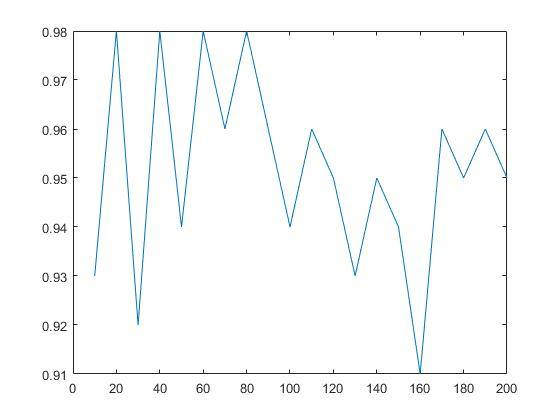
\includegraphics[width=10cm]{exercise8}
  \end{center}

  \begin{lstlisting}[style=Matlab-editor, basicstyle=\scriptsize]
    clear;
    clc;

    mu = [
        2,2;
        4,1;
        1,4;
        5,5;
        10,10;
    ];

    rng default;

    I = eye(2);
    e_mu = sum(mu)/5;

    for n=10:10:200
        count = 0;
        for i=1:100
            % Generate samples
            for j=1:n
                r = randi([1,5]);
                x(j,:) = mvnrnd(mu(r,:),I,1);
            end

            % 95% confidence region is sample mean +/- 1.96/sqrt(n) in both coordinates
            avg = mean(x);
            % variance of the mixture
            variance = 1 + 29.2 - 4.4^2;
            if ((avg(1) + 1.96*variance/sqrt(n)) > e_mu(1)) & ((avg(1) - 1.96*variance/sqrt(n)) < e_mu(1)) & ((avg(2) + 1.96*variance/sqrt(n)) > e_mu(2)) & ((avg(2) - 1.96*variance/sqrt(n)) < e_mu(2))
                count = count + 1;
            end
        end
        result(n/10) = count/100;
    end
  \end{lstlisting}
\end{answer}

\clearpage

\begin{exercise}
  Use any programming language you like to do the following.

  Consider two functions $f(x) = 4 \sin( \lVert x \rVert^2)$ and $f(x) = x_1 +x_2^2$. Let $X$ follows the Gaussian mixture specified in Exercise 8. That is, $X \sim \sum_{k = 1}^5 1/5 \cdot N(\mu_k, I_2)$. Let $Y = f(X) + \nu$, where $\nu \sim N(0,0.2)$ is independent of $X$. For each function $f$ do the following. Generate an i.i.d. training sample $\{ (x_i, y_i) \}_1^500$ of size $n=500$, and a test sample $\{ (x_i', y_i') \}_1^1000$. Let $\Delta = \max_{k,l} \lVert \mu_k - \mu_l \rVert$, and $\delta = 0.1$. Let $H$ be 20 equidistant values from $\Delta$ to $\delta$. For each $h \in H$, obtain a kernel regressor $f_h(x)$ using the training sample and the Gaussian kernel $K(u) \propto e^{- \lVert u \rVert^2/2}$. Report the error of $f_h$ by computing its mean squared error on the test sample. Plot the error of $f_h$ as a function of $h \in H$, for both $f$'s.
\end{exercise}

\begin{answer}
  Appended is the code used to generate the results. The graph of the errors are shown below. Notice that the error gets worse as the bandwidth increases. This is exactly what one would expect. For small $h$, the first function is worse in terms of error which is probably due to the sinusoidal nature of the function. Thus, the estimator needs more samples to properly estimate this function that varies much more than the quadratic function. However, as the graph suggests, for large $h$, the quadratic nature of the second function causes large errors since the furthest $\mu_k$ and $\mu_l$ is quite large ($\geq 10$).

  \begin{center}
    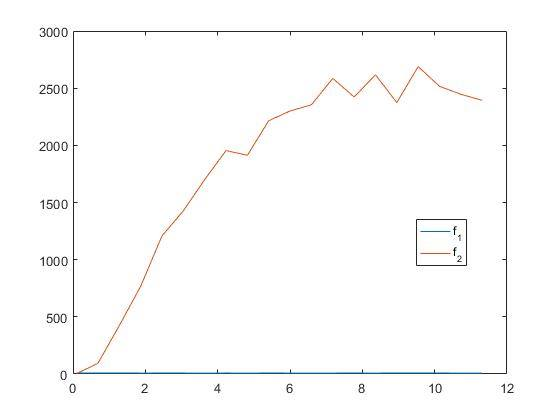
\includegraphics[width=10cm]{exercise9}
  \end{center}

  \begin{lstlisting}[style=Matlab-editor, basicstyle=\scriptsize]
    clear;
    clc;

    mu = [
        2,2;
        4,1;
        1,4;
        5,5;
        10,10;
    ];

    I = eye(2);

    rng default

    % Largest difference between mu_1 and mu_5
    Delta = sqrt(128);
    delta = 0.1;

    f_hat_1 = @(x) 0;
    f_hat_2 = @(x) 0;
    total = @(x) 0;
    H = linspace(delta, Delta, 20);

    for j = 1:20
        h = H(j);
        for i = 1:500
            % Pick Gaussian
            r = randi([1,5]);
            % Sample Gaussian
            train_sample(i,:) = mvnrnd(mu(r,:), I, 1);

            Y_1 = 4*sin(train_sample(i,1)^2 + train_sample(i,2)^2) + mvnrnd(0,0.2,1);
            Y_2 = train_sample(i,1) + train_sample(i,2)^2 + mvnrnd(0,0.2,1);

            f_hat_1 = @(x) f_hat_1(x) + exp(-((x(1)/h-train_sample(i,1)/h)^2+(x(2)/h-train_sample(i,2)/h)^2)/2)*Y_1;
            f_hat_2 = @(x) f_hat_2(x) + exp(-((x(1)/h-train_sample(i,1)/h)^2+(x(2)/h-train_sample(i,2)/h)^2)/2)*Y_2;
            total = @(x) total(x) + exp(-((x(1)/h-train_sample(i,1)/h)^2+(x(2)/h-train_sample(i,2)/h)^2)/2);
        end

        f_hat_1 = @(x) f_hat_1(x)/total(x);
        f_hat_2 = @(x) f_hat_2(x)/total(x);

        mean_square_1 = 0;
        mean_square_2 = 0;

        % test sample
        for i = 1:1000
            % Pick Gaussian
            r = randi([1,5]);
            % Sample Gaussian
            test_sample(i,:) = mvnrnd(mu(r,:), I, 1);

            Y_1 = 4*sin(test_sample(i,1)^2 + test_sample(i,2)^2) + mvnrnd(0,0.2,1);
            Y_2 = test_sample(i,1) + test_sample(i,2)^2 + mvnrnd(0,0.2,1);

            mean_square_1 = mean_square_1 + (Y_1 - f_hat_1(test_sample(i,:)))^2;
            mean_square_2 = mean_square_2 + (Y_2 - f_hat_2(test_sample(i,:)))^2;
        end

        mean_square_1 = mean_square_1/1000;
        mean_square_2 = mean_square_2/1000;

        error(j, 1) = mean_square_1;
        error(j, 2) = mean_square_2;
    end
  \end{lstlisting}
\end{answer}

\end{document}